\documentclass[12pt,a4paper]{ctexart}
\usepackage[utf8]{inputenc}
\usepackage{amsmath}
\usepackage{amsfonts}
\usepackage{amssymb}
\usepackage{makeidx}
\usepackage{graphicx}
\title{数控机床智能远程诊断暑假培训 总结}
\author{高星}
\date{}
\begin{document}
	\begin{center}
	\heiti \zihao{3}	数控机床智能远程诊断\\暑假培训总结
	
	\songti \zihao4 (高星 \hspace{1cm} 湖南九嶷职业技术学院)
	\end{center}
\indent

2017年7月16日,本人有幸参加了长沙航空职业技术学院的省培班--数控机床智能远程诊断,培训总共15天,在这紧张的培训学习过程中,我按照培训的进程,紧跟老师的思路,按时按质按量地完成了全部课题的学习,收获颇多,现总结如下。

\textbf{一 、了解了数控机床智能远程诊断的应用场合和意义}

随着数控技术的快速推广与应用,数控设备在全国已经有相当高的使用率,其经济价值得到行业的一致认同。这些设备功能强,生产效率高,但是复杂,它涉及机械、电器、液压、气动、光学、与计算机技术等许多领域,尤其在故障诊断、状态监测方面涉及数字测试技术与计算机网络技术。因此,它的维修在理论上、方法上、和手段上与普通的设备相比都有很大的区别,给维修工作带来很大的困难。一旦数控设备出现故障,哪怕是很小的问题都得停机等待维修,给企业正常的生产带来很大的影响,越来越多的企业用户希望能够最大程度降低维修和维护成本,因此,提高和改进数控设备的远程智能诊断能力,就显得尤为重要。

\textbf{二、掌握了Fanuc 远程诊断方案}

Fanuc 系统 借助于网络通信,用户既可以在远程端实时地观测机床运行现场的情况,获取被控机床的参数及特征值,又可像身临现场一样进行相应的交互式操作和控制。这样既方便了对控制对象的操作和管理,又提高了整个系统的稳定性和可靠性。

我们在以太网的基础上,搭建了Fanuc 远程诊断平台,掌握了远程诊断的流程与关键技术,我后面的学习打下了基础。

\textbf{三、提升了利用PMC进行诊断技能}

数控机床40\%的故障是由外围线路造成的,而PMC是诊断外围线路问题的关键技术,通过Fanuc 远程诊断平台,结合PMC就可以远程解决外围线路造成的故障,掌握并熟练应用PMC是远程诊断的关键,通过系统的学习Fanuc上 PMC,我们能够看懂Fanuc上MPC梯形图,并了解其工作原理,能够编写PMC梯形图,能通过结合PMC了远程诊断手轮、开关按钮、急停、进给伺服、主轴、回零、辅助功能、等故障。

\textbf{四、参观了企业了解了市场需求及发展前景}

在学习的过程我们参观了
长沙哈量凯帅精密机械有限公司及
湖南省机器人研发演示中心,
了解了本专业的市场需求及发             展前景,长沙哈量凯帅   精密机械有限公司使用Teamview远程软件应用到数控机床上,取得了非常大的成效。
湖南省机器人研发演示中心,了解了机器人专业的前景与市场,今后的维修及调试人员的需求也非常大,由于数控机床与机器人有一定的相似性,可以结合数控维修调试与机器人维修调试,提高学生的竞争力。
	
\textbf{五、提高了理实一体化教学的理念与应用}

针对数控维修这门课程的具体性,如何采用合适的教学方法也是这次培训探讨的课题。由于数控维修课程中除了需要操作实践之外,也包括了大量的理论知识,所以必须将理论和实践结合起来,两方面配合好,实现理实一体化,才能更好的让学生掌握这门课程。在培训过程中,培训的老师也是按照了这种方法来教学,在以后的教学过程中也可以学习贯彻这种理念。

\textbf{六、对自我的重新认识}

通过培训学习使我的思想有了一个新的转变,作为一位数控设备智能远程诊断技术课程教师,必须具有渊博的专业知识,熟练的操作技能,良好的思维品质,更应当掌握现代教育教学理论、掌握现代教育教学技术。在信息技术飞速发展的21世纪,我们必须加强学习,追踪行业发展新方向,掌握行业新技术。否则,我们的知识就要落后,我们培养的学生就不能适应企业的要求。


这次培训在的精心设计、安排下,培训内容生动充实、实用性强,培训教师经验丰富、精力充沛,有极强的带动性和个人魅力,教学理念先进,教学方法灵活,课堂气氛活跃,培训工作井然有序。通过本次培训,我的视野开阔了,观念转变了,理论水平与实践动手能力提高了,并结交了很多朋友和老师,丰富了自己的社会资源。我要再次感谢各位领导、各位老师为专业教师的成长所付出的辛勤劳动。衷心感谢!

\begin{figure}[h]
\begin{center}
		\includegraphics[width=0.8\linewidth]{image/1}
	\caption{教师讲解分析原理 }
\end{center}
\end{figure}

\begin{figure}[h]
	\begin{center}
		\includegraphics[width=0.8\linewidth]{image/3}
		\caption{教师操作演示数据备份}
	\end{center}
\end{figure}

\begin{figure}[h]
	\begin{center}
		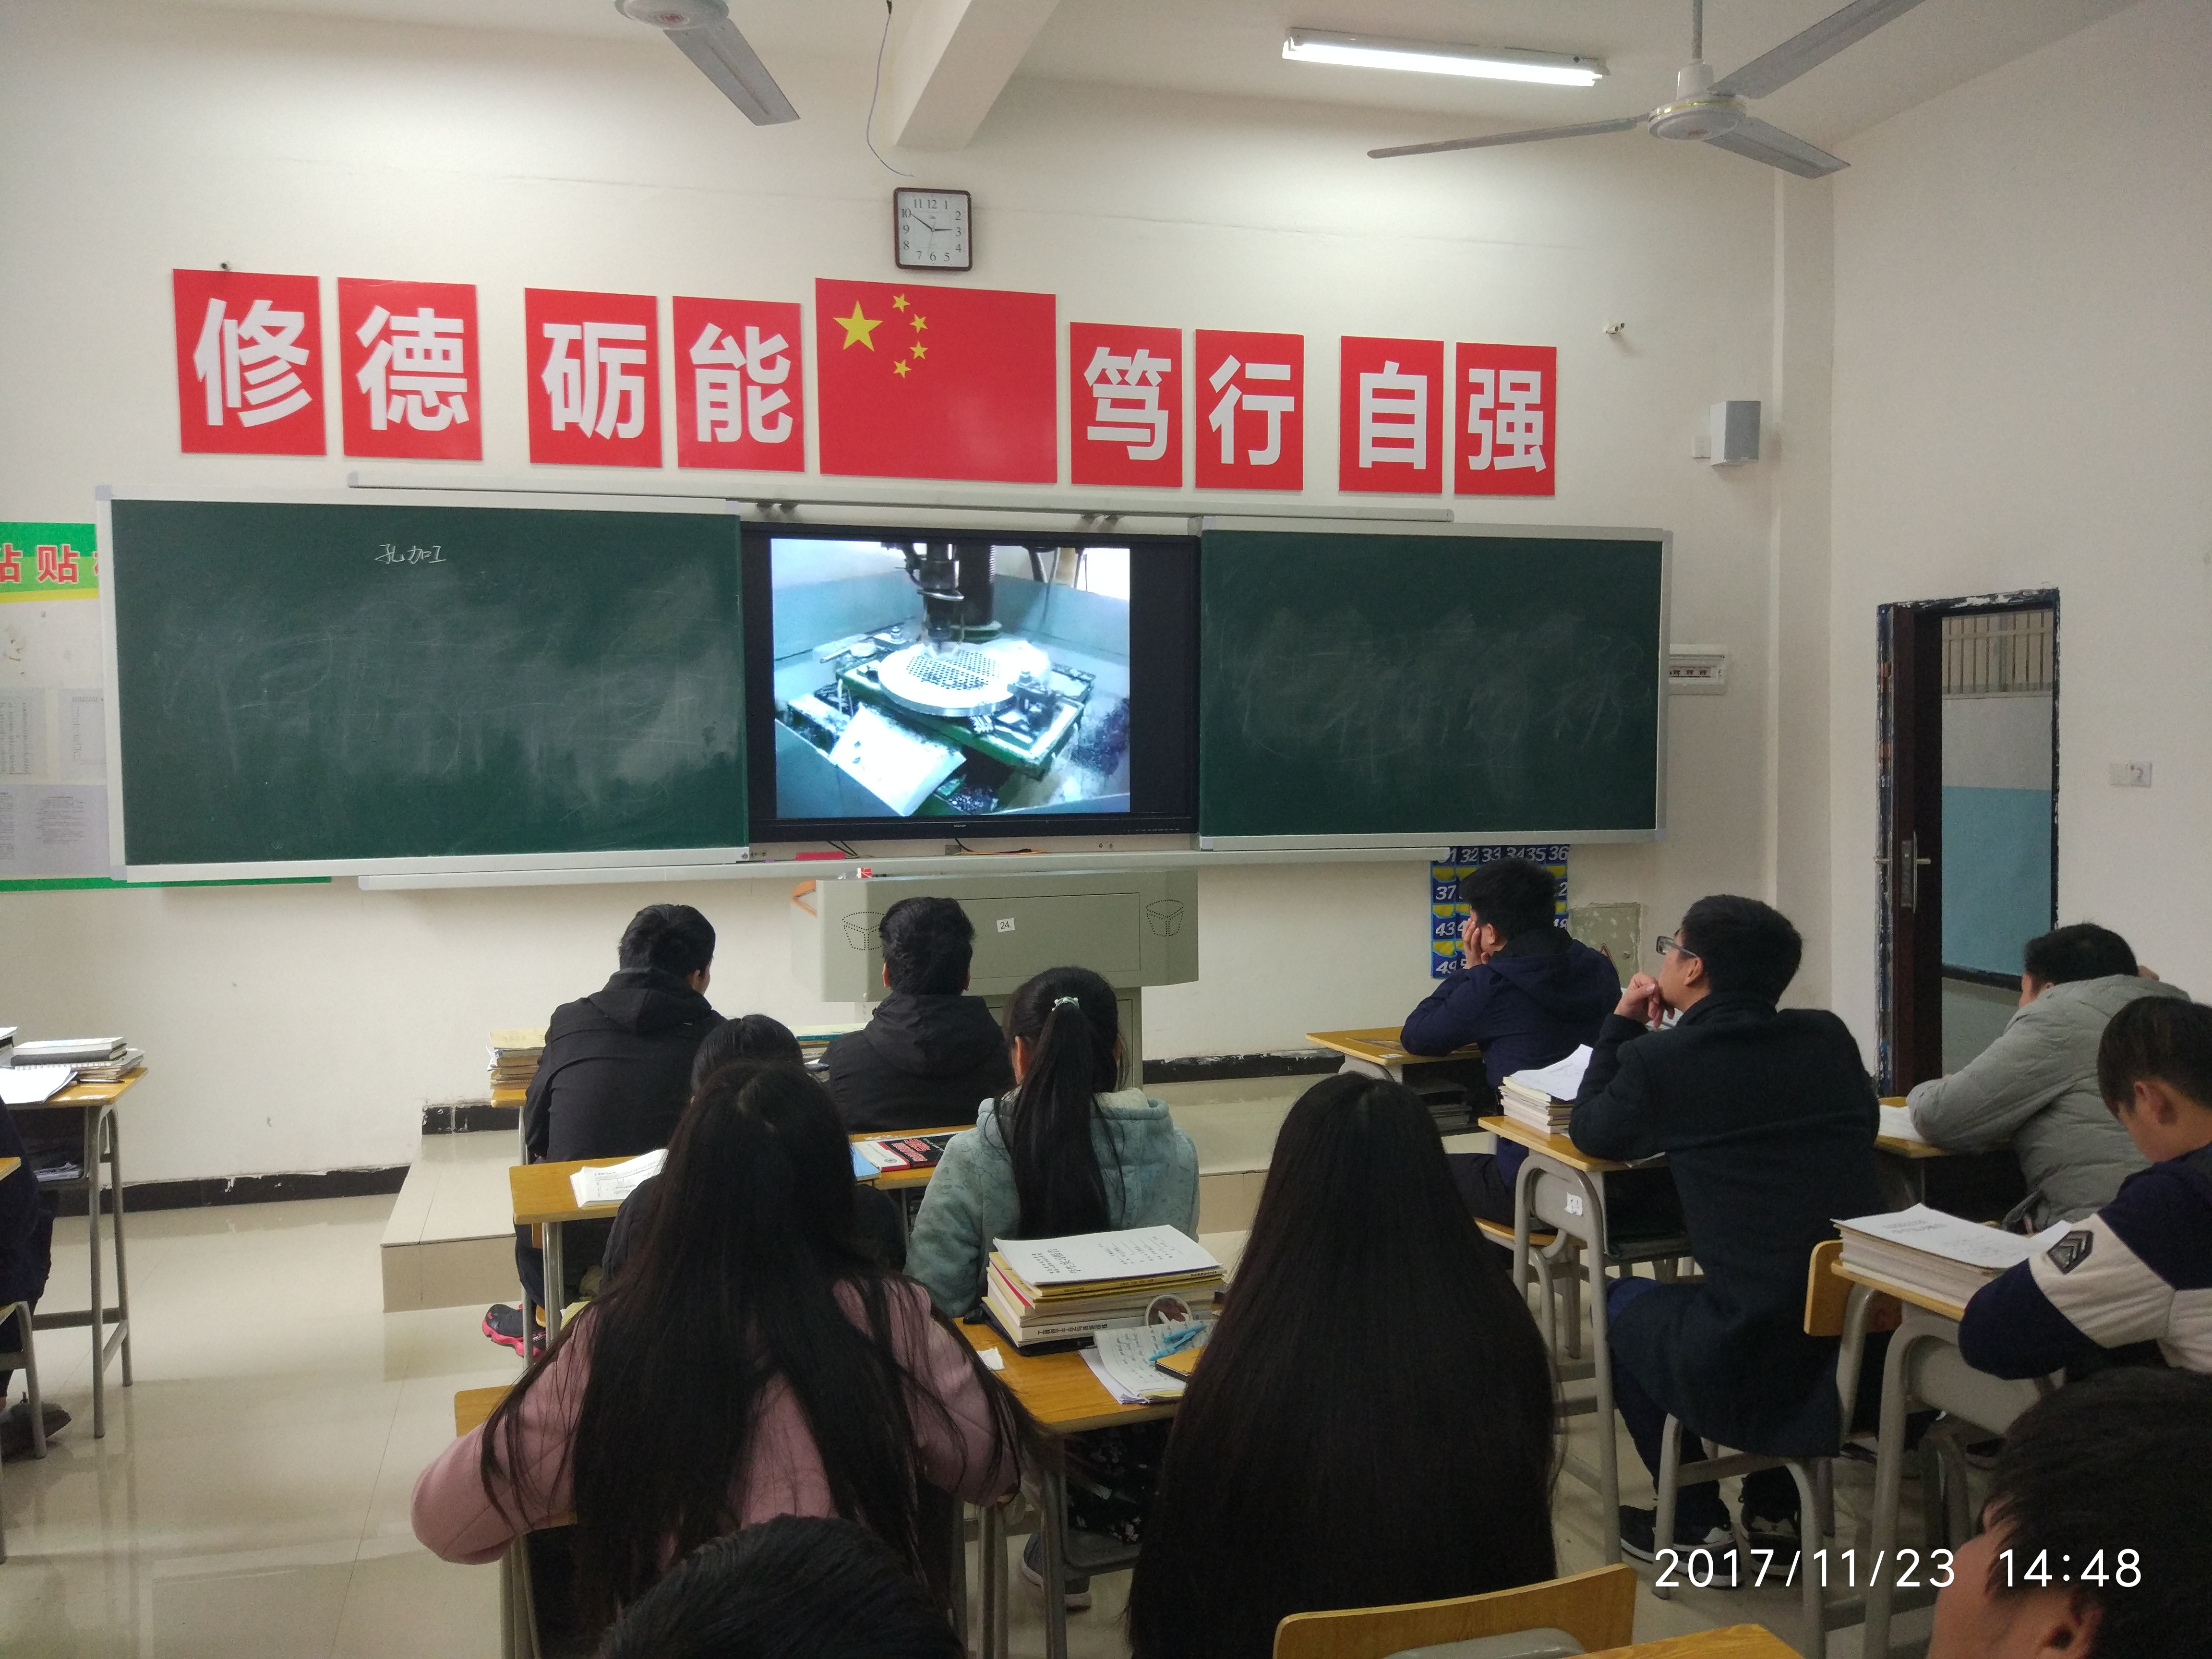
\includegraphics[width=0.8\linewidth]{image/2}
		\caption{学员拆装刀架 }
	\end{center}
\end{figure}


\begin{figure}[h]
	\begin{center}
		\includegraphics[width=0.8\linewidth]{image/4}
		\caption{学员拆装交流接触器 }
	\end{center}
\end{figure}

\begin{figure}[h]
	\begin{center}
		\includegraphics[width=0.8\linewidth]{image/5}
		\caption{学员拆装好的车床刀架 }
	\end{center}
\end{figure}

\begin{figure}[h]
	\begin{center}
		\includegraphics[width=0.8\linewidth]{image/6}
		\caption{学员拆装好的行程开关}
	\end{center}
\end{figure}

\begin{figure}[h]
	\begin{center}
		\includegraphics[width=0.8\linewidth]{image/7}
		\caption{企业参观 }
	\end{center}
\end{figure}

\begin{figure}[h]
	\begin{center}
		\includegraphics[width=0.8\linewidth]{image/8}
		\caption{企业参观 }
	\end{center}
\end{figure}

\begin{figure}[h]
	\begin{center}
		\includegraphics[width=0.8\linewidth]{image/9}
		\caption{市场调查与交流 }
	\end{center}
\end{figure}

\begin{figure}[h]
	\begin{center}
		\includegraphics[width=0.8\linewidth]{image/10}
		\caption{企业车间 }
	\end{center}
\end{figure}

\begin{figure}[h]
	\begin{center}
		\includegraphics[width=0.8\linewidth]{image/11}
		\caption{学员课外活动 }
	\end{center}
\end{figure}

\begin{figure}[h]
	\begin{center}
		\includegraphics[width=0.8\linewidth]{image/12}
		\caption{全体学员留影}
	\end{center}
\end{figure}

\end{document}